\chapter{Background and Related Works}


\section{Maps}

\begin{definition}
    A map is said to be \textbf{nomad} when the players will start with no towncenter, and some villagers. Each player is required to create a town center wherever she desires.
\end{definition}

\begin{definition}
    A map is said to be \textbf{michi} the players will be separated by forest.
\end{definition}

Cliffs (see \defref{def:cliff}) are another element on the map. A cliff is shown in \figref{fig:cliff}

\begin{definition}\label{def:cliff}
    A cliff is an untraversable element of the map. Units on the cliff gain a strategic advantage \wrt{} unit under the cliff.
\end{definition}

\begin{figure}[ht]
    \centering
    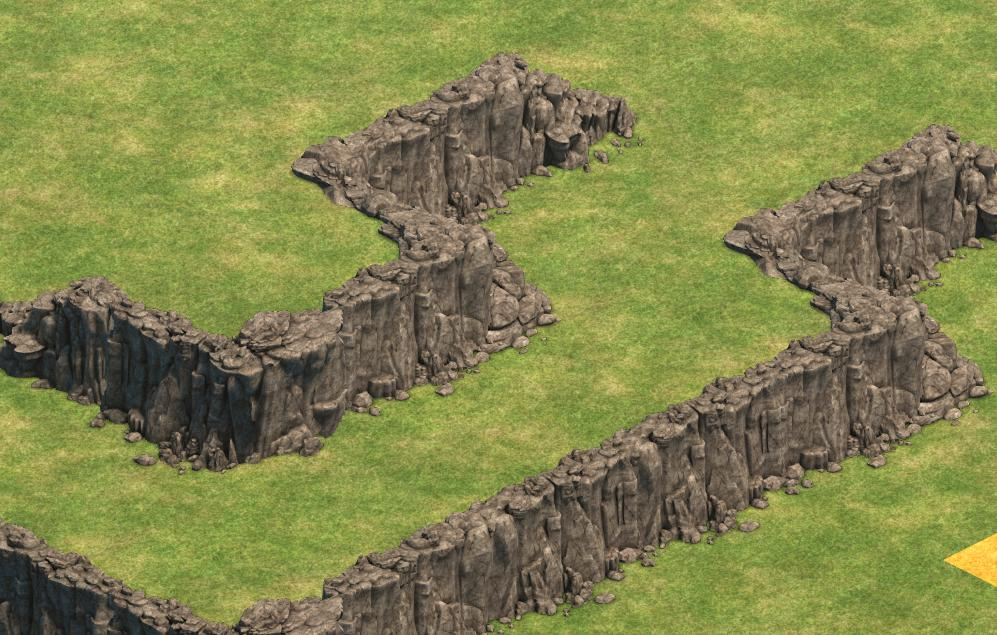
\includegraphics[width=0.8\textwidth]{src/images/cliffs}
    \caption{Example of a cliff in a map.}
    \label{fig:cliff}
\end{figure}

Maps have fixed \textbf{sizes}, which are shown in \tblref{tbl:size}\cite{zetnus:2015}.

\begin{table}[ht]
    \centering
    \begin{tabular}{llll}
        \toprule
        Size & Tiles on Sides & Total tiles & Area ratio to 100x100 map \\
        \midrule
        Tiny        & 120x120              & 14400           & 1.4 \\
        Small       & 144x144              & 20736           & 2.1 \\
        Medium      & 168x168              & 28224           & 2.8 \\
        Large       & 200x200              & 40000           & 4.0 \\
        Huge        & 220x220              & 48400           & 4.8 \\
        Gigantic    & 240x240              & 57600           & 5.8 \\
        Ludicruous  & 480x480              & 230400          & 23.0 \\
        \bottomrule
    \end{tabular}
    \caption{Allowed map sizes.}
    \label{tbl:size}
\end{table}

\subsection{Types of maps}

You can play \aoe{} on several different maps. A map can be played with a specific playstyle. The types of maps are the following ones:

\begin{itemize}
    \item Random Maps
    \item Death Match;
    \item Battle Royale;
    \item King of the Hill;
\end{itemize}

\figref{fig:aoe:maps} shows some maps available to play in \aoe{}.

\begin{figure}
    \begin{subfigure}{0.22\textwidth}
        \centering
        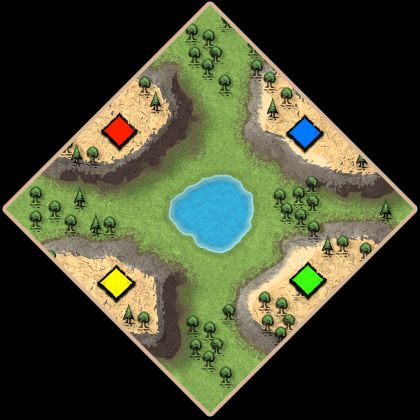
\includegraphics[width=1.0\textwidth]{src/images/maps/rm-acropolis}
        \caption{Acropolis}
    \end{subfigure}\quad%
    \begin{subfigure}{0.22\textwidth}
        \centering
        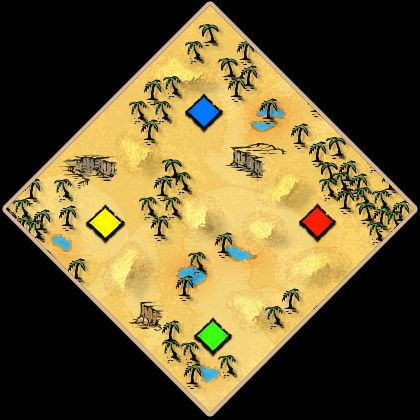
\includegraphics[width=1.0\textwidth]{src/images/maps/rm-arabia}
        \caption{Arabia}
    \end{subfigure}\quad%
    \begin{subfigure}{0.22\textwidth}
        \centering
        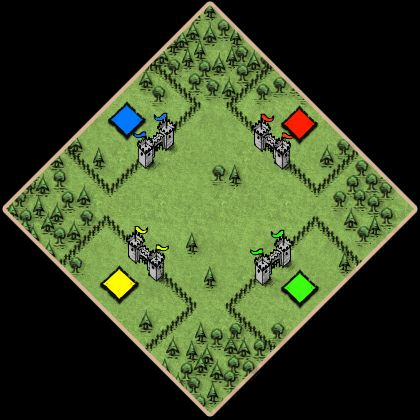
\includegraphics[width=1.0\textwidth]{src/images/maps/rm-arena}
        \caption{Arena}
    \end{subfigure}\quad%
    \begin{subfigure}{0.22\textwidth}
        \centering
        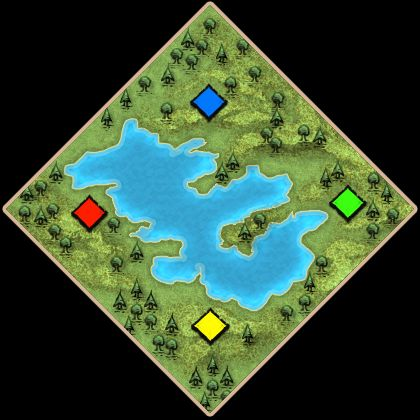
\includegraphics[width=1.0\textwidth]{src/images/maps/rm-baltic}
        \caption{Baltic}
    \end{subfigure}\\%
    %
    \begin{subfigure}{0.22\textwidth}
        \centering
        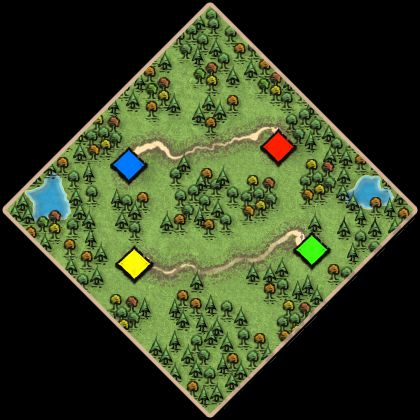
\includegraphics[width=1.0\textwidth]{src/images/maps/rm-black-forest}
        \caption{Black Forest}
    \end{subfigure}\quad%
    \begin{subfigure}{0.22\textwidth}
        \centering
        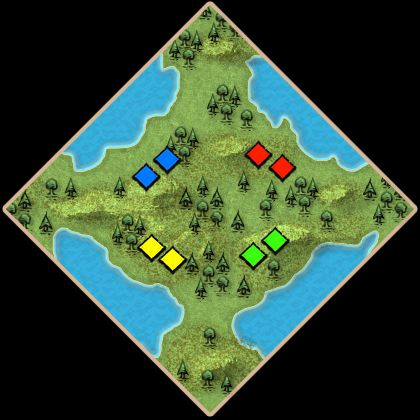
\includegraphics[width=1.0\textwidth]{src/images/maps/rm-budapest}
        \caption{Budapest}
    \end{subfigure}\quad%
    \begin{subfigure}{0.22\textwidth}
        \centering
        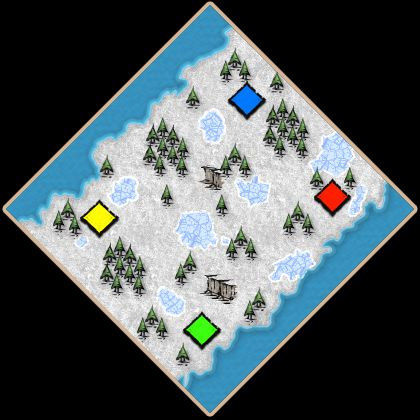
\includegraphics[width=1.0\textwidth]{src/images/maps/rm-scandinavia}
        \caption{Scandinavia}
    \end{subfigure}\quad%
    \begin{subfigure}{0.22\textwidth}
        \centering
        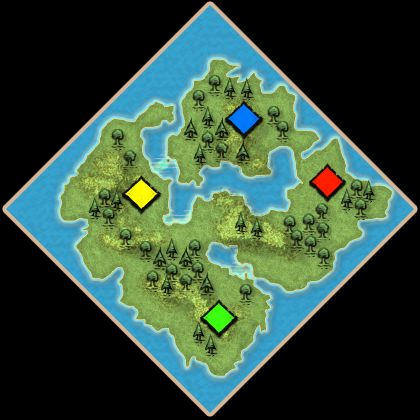
\includegraphics[width=1.0\textwidth]{src/images/maps/rm-continental}
        \caption{Continental}
    \end{subfigure}\\%
    % %
    % \begin{subfigure}{0.24\textwidth}
    %     \centering
    %     \includegraphics[1.0\textwidth]{src/images/maps/}
    %     \caption{}
    % \end{subfigure}%
    % \begin{subfigure}{0.24\textwidth}
    %     \centering
    %     \includegraphics[1.0\textwidth]{src/images/maps/}
    %     \caption{}
    % \end{subfigure}%
    % \begin{subfigure}{0.24\textwidth}
    %     \centering
    %     \includegraphics[1.0\textwidth]{src/images/maps/}
    %     \caption{}
    % \end{subfigure}%
    % \begin{subfigure}{0.24\textwidth}
    %     \centering
    %     \includegraphics[1.0\textwidth]{src/images/maps/}
    %     \caption{}
    % \end{subfigure}\\%
    % %
    % \begin{subfigure}{0.24\textwidth}
    %     \centering
    %     \includegraphics[1.0\textwidth]{src/images/maps/}
    %     \caption{}
    % \end{subfigure}%
    % \begin{subfigure}{0.24\textwidth}
    %     \centering
    %     \includegraphics[1.0\textwidth]{src/images/maps/}
    %     \caption{}
    % \end{subfigure}%
    % \begin{subfigure}{0.24\textwidth}
    %     \centering
    %     \includegraphics[1.0\textwidth]{src/images/maps/}
    %     \caption{}
    % \end{subfigure}%
    % \begin{subfigure}{0.24\textwidth}
    %     \centering
    %     \includegraphics[1.0\textwidth]{src/images/maps/}
    %     \caption{}
    % \end{subfigure}\\%
    % %
    % \begin{subfigure}{0.24\textwidth}
    %     \centering
    %     \includegraphics[1.0\textwidth]{src/images/maps/}
    %     \caption{}
    % \end{subfigure}%
    % \begin{subfigure}{0.24\textwidth}
    %     \centering
    %     \includegraphics[1.0\textwidth]{src/images/maps/}
    %     \caption{}
    % \end{subfigure}%
    % \begin{subfigure}{0.24\textwidth}
    %     \centering
    %     \includegraphics[1.0\textwidth]{src/images/maps/}
    %     \caption{}
    % \end{subfigure}%
    % \begin{subfigure}{0.24\textwidth}
    %     \centering
    %     \includegraphics[1.0\textwidth]{src/images/maps/}
    %     \caption{}
    % \end{subfigure}\\
    \caption{Examples of maps available in \aoe{}. Red, Yellow, Green and Blue diamond represents players positions. If a team game is played, Red and blue are allied against team yellow and green. A shoe represents a nomadic map. }
    \label{fig:aoe:maps}
\end{figure}